%%%%%%%%%%%%%%%%%%%%%%%%%%%%%%%%%%%%%%%%%%%%%%
%                insertmeeting
% 1) Title (something creative & funny?)
% 2) Date (MM/DD/YYYY)
% 3) Location (ex. Hagerty High School)
% 4) People/Committees Present 
% 5) Picture 
% 6) Start Time & Stop Time (ex. 12:30AM to 4:30PM)
%%%%%%%%%%%%%%%%%%%%%%%%%%%%%%%%%%%%%%%%%%%%%%
\insertmeeting 
	{After Christmas, Before New Years} 
	{12/28/21} 
	{Hagerty High School}
	{Jensen, Nathan, Ritam}
	{Images/RobotPics/robot.jpg}
	{2:30 - 4:30}
	
\hhscommittee{Hardware}
\noindent\hfil\rule{\textwidth}{.4pt}\hfil
\subsubsection*{Goals}
\begin{itemize}
    \item 3D print new intake
    \item Test belt distances
    \item Start building intake
  

\end{itemize} 

\noindent\hfil\rule{\textwidth}{.4pt}\hfil

\subsubsection*{Accomplishments}
After a long hiatus from the intake, today is the day that we once again take our design from CAD into the real world, but this time, it will be printed out of nylon from a printer in UCF’s Innovation lab, which will make the intake much stronger than before. Despite the strength of nylon, we decided to print the intake unpocketed, thinking its pocketing would only save a few grams of weight and wouldn’t be worth the sacrifice of strength. After coming back later and seeing the print, we were surprised to see that it was heavier than we had originally estimated based on onshape’s mass finding tools. Weighing in at about 56 grams (Figure \ref{fig:122821_1}), the intake was still pretty light, but not light enough to make our decision to take out the pocketing holes fully worth it. Looking at the print, we found some other errors. Aside from having poor print quality caused by poor print settings, the hole where the shaft would connect was too small for the graphite pole we planned on using to fit into. Although none of these issues are detrimental on their own, we decided to reprint, especially because we didn’t even think we could finish today anyway. Quickly going into CAD and making the needed revisions, we started printing again, this time with settings that will hopefully give us a smoother final product. Although this means we can’t start building the intake until the next meeting when the revised version is done printing, we still used this version to make sure all of the belts and pulleys would fit well together. This proved to be useful, as we were able to confirm that the reprint we had just started had the correct dimensions for the pulleys and belts to fit properly.


\begin{figure}[htp]
\centering
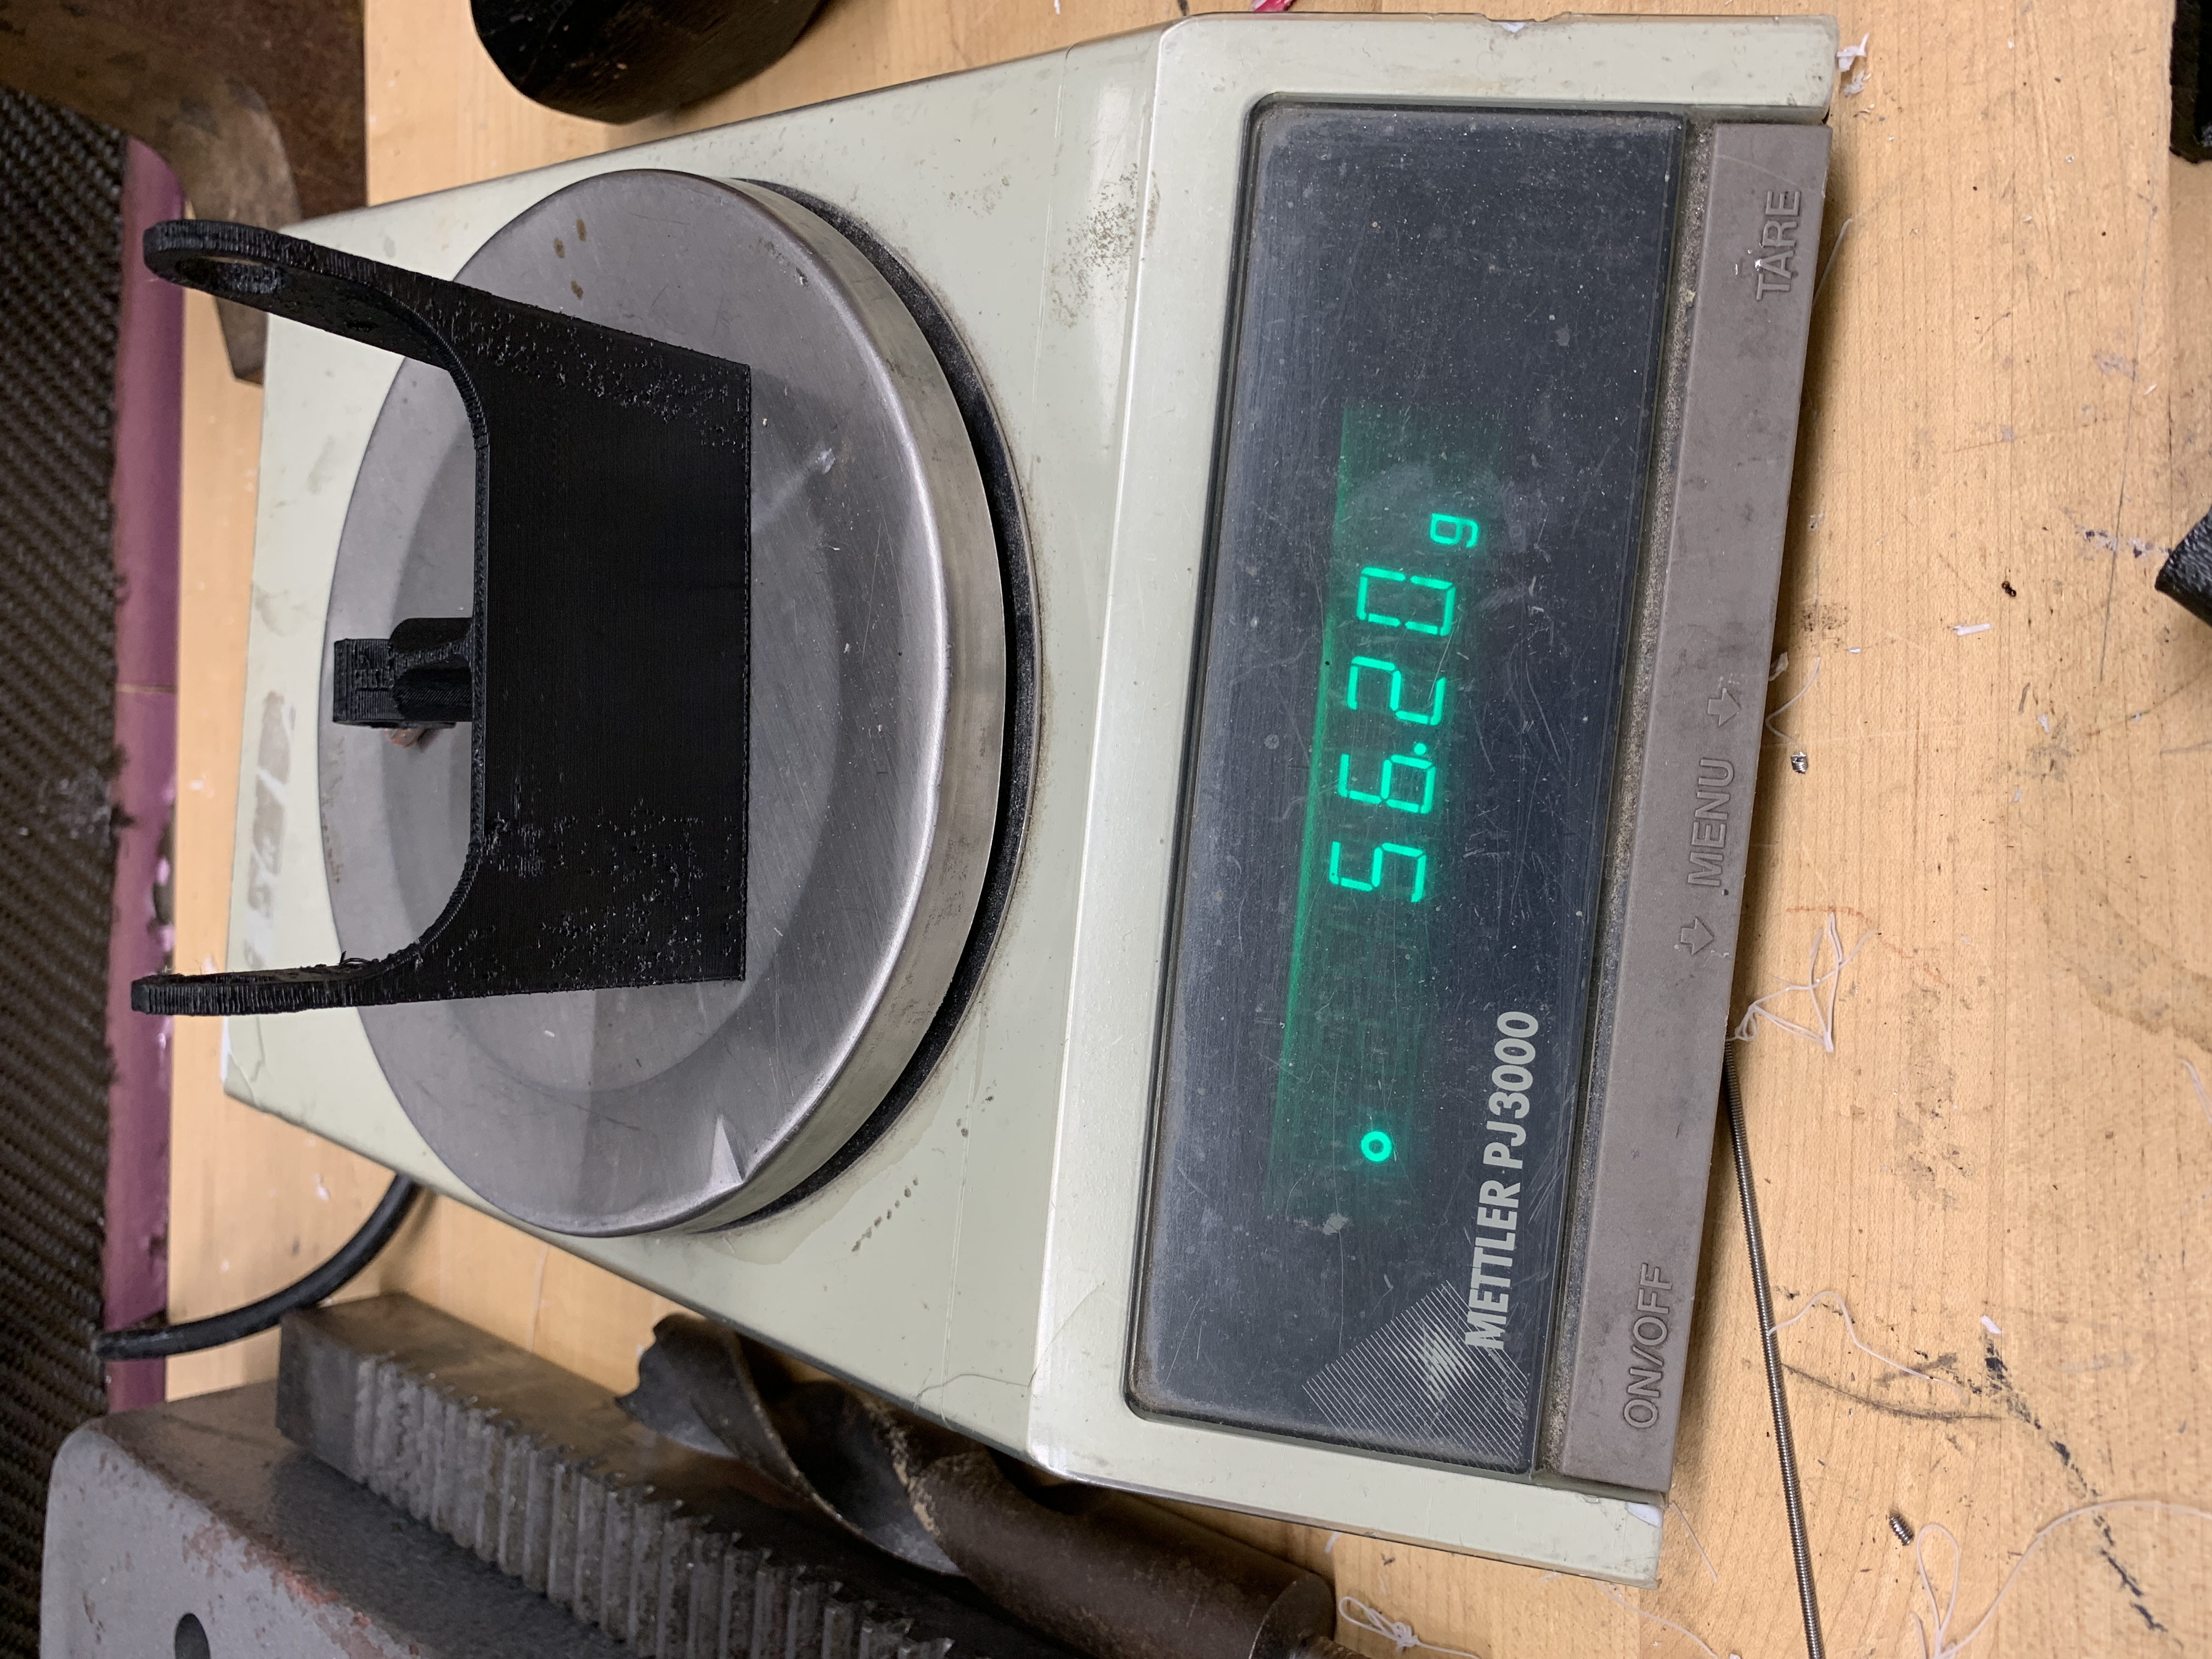
\includegraphics[width=0.95\textwidth, angle=0]{Meetings/December/12-28-21/12-28-21_Hardware_Figure1 - Nathan Forrer.JPG}
\caption{The intake was heavier than expected}
\label{fig:122821_1}
\end{figure}


\whatsnext{
\begin{itemize}
    \item Print adjusted intake
    \item Build new roller intake
    \item Test new roller intake.

\end{itemize} 
}

